\documentclass[12pt,aspectratio=169]{beamer}
\input{../../mybeamer}
\usetikzlibrary{patterns}


\title{Classes 3 \& 4: Gauss's Law}
\subtitle{AP Physics C: Electricity and Magnetism}
\input{../../me}
\input{../../mycommands}


\begin{document}

\begin{frame}
  \maketitle
\end{frame}


\section{Gauss's Law}

\begin{frame}{Flux}
  \textbf{Flux} is an important concept in many disciplines in physics. The
  flux of a vector quantity $\vec X$ is the amount of that quantity flowing
  through a surface. In integral form:

  \eq{-.1in}{
    \Phi=\int_{\mathcal S}\vec X\cdot\dl\vec A\quad\text{or}\quad
    \Phi=\int_{\mathcal S}(\vec X\cdot\hat n)\dl A
  }

  The direction of the infinitesimal area $\dl\vec A$ is \textbf{outward normal}
  to the surface.
  \begin{center}
    \pic{.3}{eflux}
  \end{center}
\end{frame}



\begin{frame}{Flux}
  \vspace{.2in}$\Phi$ can be something physical, like water, or bananas, or
  something abstract, like electric field (which is what we are interested
  in). We can compute a flux as long as there is a vector field i.e.\
  $\vec X=\vec X(x,y,z)$. In the case of \textbf{electric flux}, the quantity
  $\vec X$ is just the electric field, i.e.:
    
  \eq{-.1in}{
    \boxed{ \Phi_E=\int\vec E\cdot\dl\vec A }
  }
  \begin{center}
    \pic{.3}{eflux}
  \end{center}
\end{frame}



\begin{frame}{Electric Flux and Gauss's Law}
  \textbf{Gauss's law} tells us that for a closed surface $\mathcal S$ (think
  of the surface of a balloon), the total electric flux is given by:

  \eq{-.1in}{
    \boxed{
      \Phi_E=\oint_{\mathcal S}\vec E\cdot\dl\vec A
      =\frac{Q_\text{encl}}{\epsilon_0}
    }
  }
    
  where
  \begin{itemize}
  \item $Q_\text{encl}$ is the charge enclosed by the surface
  \item $\epsilon_0=\SI{8.85e-12}{C^2/N.m^2}$ is the permittivity of free space
  \end{itemize}
  That closed surface is called a \textbf{Gaussian surface}
\end{frame}



\begin{frame}{Closed Surfaces}
  \begin{columns}
    \column{.55\textwidth}
    A \textbf{closed surface} is one that does not have a boundary, like the
    sphere, toroid, and cube on the left.
    \column{.45\textwidth}
    \pic1{800px-SurfacesWithAndWithoutBoundary}
  \end{columns}
\end{frame}



\begin{frame}{Gauss's Law}
  \begin{center}
    \begin{tikzpicture}[scale=.37]
      \node (0) at (-4.25, 0.75) {};
      \node (1) at (-2.25, 1) {};
      \node (2) at (-4.5, -0.25) {};
      \node (3) at (-2.5, -0.25) {};
      \node (4) at (1.25, 1.75) {};
      \node (5) at (-0.75, 3) {};
      \node (6) at (-5.5, 3) {};
      \node (7) at (-7.5, 0.25) {};
      \node (8) at (-5.25, -2.5) {};
      \node (9) at (0, -1) {};
      \node (10) at (4.25, 4.25) {};
      \node (11) at (-2.5, 5.25) {};
      \node (12) at (-9.75, 4.75) {};
      \node (13) at (-10.75, -1) {};
      \node (15) at (-3, -5) {};
      \node (16) at (4.5, -1) {};
      
      \draw[very thick,pattern=north east lines] (1.center)
      to[in=45, out=-180, looseness=1.5] (0.center)
      to[in=135, out=-135, looseness=0.75] (2.center)
      to[in=165, out=-60, looseness=0.75] (3.center)
      to[in=0, out=-15, looseness=1.25] (1.center);
  
      \shade[ball color=orange,opacity=.7] (5.center)
      to[in=15,out=-150] (6.center)
      to[in=105,out=-165] (7.center)
      to[in=180,out=-75] (8.center)
      to[in=165,out=0,looseness=1.25] (9.center)
      to[in=-75,out=0] (4.center)
      to[in=30,out=105,looseness=.75] (5.center);

      \draw[thick,orange] (5.center)
      to[in=15,out=-150] (6.center)
      to[in=105,out=-165] (7.center)
      to[in=180,out=-75] (8.center)
      to[in=165,out=0,looseness=1.25] (9.center)
      to[in=-75,out=0] (4.center)
      to[in=30,out=105,looseness=.75] (5.center);
    
      \begin{scope}[vectors,orange]
        \draw (-5,2.5)--+(-.5,1.7);
        \draw (-4,2.5)--+(-.3,2);
        \draw (-3,2.5)--+(.1,2) node[right]{$\bm E$};
        \draw (-2,2.2)--+(.4,1.8);
        \draw (-1,2.35)--+(.7,1.8);
      \end{scope}
    
      \shade[ball color=violet,opacity=.2] (10.center)
      to[in=0,out=150,looseness=1.50] (11.center)
      to[in=30,out=-180] (12.center)
      to[in=90,out=-150,looseness=1.5] (13.center)
      to[in=150,out=-90,looseness=1.25] (15.center)
      to[in=-90,out=-30,looseness=.75] (16.center)
      to[in=-30,out=90,looseness=.75]  (10.center);
      
      \draw[thick,violet] (10.center)
      to[in=0,out=150,looseness=1.50] (11.center)
      to[in=30,out=-180] (12.center)
      to[in=90,out=-150,looseness=1.5] (13.center)
      to[in=150,out=-90,looseness=1.25] (15.center)
      to[in=-90,out=-30,looseness=.75] (16.center)
      to[in=-30,out=90,looseness=.75]  (10.center);

      \begin{scope}[vectors,violet]
        \draw (-9.75,4.4)--+(-.5,.6);
        \draw (-8,5.1)--+(-.4,.8);
        \draw (-6,5.3)--+(-.3,.8) node[right]{$\bm E$};
        \draw (-4,5.2)--+(-.2,.7);
        \draw (-2,5.1)--+(.1,.8);
        \draw (0,5.2)--+(.2,.6);
        \draw (2,5.2)--+(.4,.5);
      \end{scope}
      \draw[thick] (-3.3,.5) to[out=270,in=90] +(2,-2)
      node[below]{$Q_\text{encl}$};
      \node[right,violet] at (4.3,4.3) {$\mathcal S_2$};
      \node[right,orange] at (1.3,1.8) {$\mathcal S_1$};
    \end{tikzpicture}
  \end{center}
  \vspace{-.1in}Two Gaussian surfaces over the same enclosed charge have the
  same total flux:
  \begin{itemize}
  \item $\mathcal S_1$ has a smaller surface for integration and stronger
    electric field
  \item $\mathcal S_2$ has a larger surface, but weaker electric field
  \end{itemize}
%  But,
%
%  \eq{-.2in}{
%    \oint_{\mathcal S_1}\vec E\cdot\dl\vec A
%    = \oint_{\mathcal S_2}\vec E\cdot\dl\vec A
%    =\frac{Q_\text{encl}}{\epsilon_0}
%  }
\end{frame}



\begin{frame}{Electric Field from a Positive Point Charge}
  \begin{columns}
    \column{.35\textwidth}
    \begin{tikzpicture}[scale=1.2]
      \foreach \x in {1,...,12}{
        \draw[red!65!black,axes,rotate=30*\x] (0,0)--(0,1);
        \draw[red!65!black,thick,rotate=30*\x] (0,0)--(0,2);
      }
      \shade[ball color=red!70!black] circle (.08);
      \node[red!65!black,right] at (2,0) (E) {$\vec E$};
      \uncover<2>{
        \shade[ball color=blue,opacity=.5] circle (1.5);
        \draw[axes] (0,1.5)--(0,2) node[above]{$\hat n$};
      }
    \end{tikzpicture}
    
    \column{.65\textwidth}
    By symmetry, electric field lines must be radially outward from the charge,
    so the integral reduces to:

    \eq{-.1in}{
      \Phi_E=\oint_{\mathcal S}\vec E\cdot\dl\vec A=EA=\frac q{\epsilon_0}
    }

    Since area of a sphere is $A=4\pi r^2$, we recover Coulomb's law and the
    magnitude of the electric field from a point charge:

    \eq{-.1in}{
      E=\frac1{4\pi\epsilon_0}\frac q{r^2}=\frac{kq}{r^2}
    }
  \end{columns}
\end{frame}



\begin{frame}{Uniformly-Charged Thin Shell}
  For a uniformly-charged spherical thin shell with radius $R$ and a total
  charge of $Q$.
  
  \vspace{.1in}
  \begin{columns}
    \column{.28\textwidth}
    \centering
    \begin{tikzpicture}[scale=.9]
      \draw[thick,fill=black!70] circle (1.5);
      \draw[thick,fill=black!2] circle (1.45);
      \draw[axes,rotate=60] (0,0)--(1.5,0) node[above]{$R$};
      \uncover<1>{
        \shade[ball color=red,opacity=.7] circle (1.5);
      }
      \uncover<2>{
        \draw[axes,rotate=-20] (0,0)--(1,0) node[midway,below]{$r_i$};
        \draw[dashed,gray,thick] circle (1);
      }

      \uncover<3>{
        \draw[axes,rotate=-20] (0,0)--(2.25,0) node[pos=.4,below]{$r_0$};
        \draw[dashed,gray,thick] circle (2.25);
      }
    \end{tikzpicture}
    
    \column{.72\textwidth}

    \uncover<2->{
      Inside the shell ($r_i<R$), there is no enclosed charge, therefore
      the electric field must be zero:
      
      \eq{-.1in}{
        \oint_{\mathcal S}\vec E\cdot\dl\vec A=\frac{q_\text{encl}}{\epsilon_0}=0
        \quad\rightarrow\quad E=0
      }
    }

    \uncover<3>{
      Outside the shell ($r_0>R$), the enclosed charge is
      $Q$, and the electric field is given by the same equation as the point
      charge:
      
      \eq{-.15in}{
        \oint_{\mathcal S}\vec E\cdot\dl\vec A=\frac Q{\epsilon_0}
        \;\rightarrow\; E=\frac Q{\epsilon_0A}
        =\frac1{4\pi\epsilon_0}\left[\frac Q{r^2}\right]
      }
    }
  \end{columns}
\end{frame}



\begin{frame}{Uniformly-Charged Thin Shell}
  The electric field strength $E$ can be plotted as a function of the distance
  $r$ from the center of the shell:
  \begin{center}
    \begin{tikzpicture}
      \draw[axes] (0,0)--(0,3) node[right]{$E$};
      \draw[axes] (0,0)--(5.5,0) node[right]{$r$};
      \draw[dashed] (1,0)--(1,2) node[pos=0,below]{$R$}
      --(0,2) node[left]{$\dfrac1{4\pi\epsilon_0}\dfrac Q{R^2}$};
      \draw[functions,smooth,domain=1:5] plot(\x,{2/\x});
      \draw[functions] (0,0)--(1,0);
      \draw[functions,fill=black!2] (1,0) circle (.06);
      \fill[red!80!black] (1,2) circle (.06);
    \end{tikzpicture}
  \end{center}
  \begin{itemize}
  \item This graph may be familiar because the graph for the gravitational field
    strength inside a uniform shell is exactly the same
  \item For gravity, replace $\epsilon_0$ with $4\pi G$
  \end{itemize}
\end{frame}



\begin{frame}{Electric Fields from a Uniformly-Charged Sphere}
  \textbf{Example:} Consider a uniformly-charged sphere with radius $R$ and a
  total charge of $Q$. The charge is evenly spread over the entire volume of
  the sphere.
  \begin{center}
    \begin{tikzpicture}[scale=.6]
      \foreach \x in {0,15,...,359}{
        \draw[orange,vectors,rotate=\x] (0,1.5)--+(0,1);
        \draw[orange,very thick,rotate=\x] (0,1.5)--+(0,1.5);
      }
      \draw[thick,red] circle (1.5);
      \shade[ball color=red,opacity=.6] circle (1.5);
      
      \draw[axes] (0,0)--(1,0) node[right]{$r_i$};
      \draw[dashed,thick] circle (1);

      \draw[axes,rotate=-50] (0,0)--(2.4,0) node[below]{$r_o$};
      \draw[dashed,thick] circle (2.4);
    \end{tikzpicture}
    %\caption{Gaussian surfaces inside and outside a spherical charge.}
    %\label{fig:uniform-spherical-charge}
  \end{center}
  Again, we are interested in the electric field inside ($r_i<R$) and outside
  ($r_o>R$) the sphere. To analyis the electric field, we contruct two spherical
  Gaussian surfaces concentric with the sphere, one inside and one outside the
  sphere.
\end{frame}




\begin{frame}{Infinitely-long charge rod with uniform density}
  \textbf{Example:} Find the electric fields inside and outside an
  infinitely-long charged rod of radius $R$ with uniform charge density.
  In this example, since the rod is infinitely long, the total charge would be
  infinite, it would be easier to describe the charge by its charge density
  $\rho$.
  \begin{center}
    \begin{tikzpicture}[scale=.45]
      \draw[thick,dashed,violet,fill=violet!30,opacity=.2] (0,2.8)--(8,2.8)
      arc (90:270:1.4 and 2.8)--(0,-2.8) arc(270:90:1.4 and 2.8);

      \draw[thick,fill=lightgray] ellipse (1 and 2);

      \draw[thick,dashed,magenta,fill=magenta!30,opacity=.3] (0,1)--(8,1)
      arc (90:270:.5 and 1)--(0,-1) arc(270:90:.5 and 1);
      \draw[thick,dashed,magenta,fill=magenta!50,opacity=.3] (0,1)--(8,1)
      arc (90:-90:.5 and 1)--(0,-1) arc(-90:90:.5 and 1);
      
      \draw[thick,fill=gray] (0,2)--(8,2) arc (90:-90:1 and 2)--(0,-2)
      arc (-90:90:1 and 2);

      \draw[thick] (-5,0)--(0,0);
      \draw[thick] (9,0)--(11,0);
      \draw[thick,dashed] (-5,2)--(11,2);
      \draw[thick,dashed] (-5,-2)--(11,-2);
      \draw[thick,dashed,violet] ellipse (1.4 and 2.8);
      \draw[thick,dashed,violet,fill=violet!50,opacity=.2] (0,2.8)--(8,2.8)
      arc (90:-90:1.4 and 2.8)--(0,-2.8) arc(-90:90:1.4 and 2.8);
      \foreach \x in {0,...,8}{
        \draw[vectors,orange!50] (\x,2.8)--(\x,4.1);
        \draw[vectors,orange!50] (\x,-2.8)--(\x,-4);
      }
      \draw[violet] (7.5,-2.8)--(6,-5) node[left]{Gaussian surface};
    \end{tikzpicture}
  \end{center}
\end{frame}


\begin{frame}{Infinitely-long charge rod with uniform density}
%  \end{subfigure}
  \begin{center}
    \begin{tikzpicture}[scale=.6]
      \draw[thick,fill=lightgray] circle (2);
      \fill circle (.05);

      \foreach \x in {0,30,...,359}{
        \draw[orange,vectors,rotate=\x] (0,0)--(0,1.8);
        \draw[orange,very thick,rotate=\x] (0,0)--(0,2);
        \draw[orange!50,vectors,rotate=\x] (0,2)--(0,4);
      }
      \draw[axes,rotate=-45] (0,0)--(2,0) node[right]{$R$};
      \draw[thick,dashed,magenta] circle (1);
      \draw[thick,dashed,violet] circle (2.8);
      \begin{scope}[rotate=-110,violet]
        \draw[axes] (0,0)--(2.8,0) node[right]{$r_o$};
        \draw (0,0)--(5,0) node[right]{Gaussian surface};
      \end{scope}
    \end{tikzpicture}
  \end{center}
  By symmetry, the electric field must only have a outward/inward radial
  component, and no component along the axial direction.
%  \caption{Infinitely-Long charged rod with uniform charge density}
%  \label{fig:charged-rod}
\end{frame}

  
%
%\textbf{Inside the rod:} By symmetry, the electric field must only be in the
%radial direction: radially outward if the rod is positively charged, and
%radially inward if negative. Here we assume that the rod is positively charged.
%We then contruct a cylindrical Gaussian surface with radius $r_i<R$ and length
%$L$ that aligns with the axis of the rod. Since the electric field is radial,
%there is no flux through the ends of the Gaussian surface, only through the
%side. The total charge enclosed by the Gaussian surface is:
%\begin{equation*}
%  q_\text{encl}=\rho V_\text{encl}=\rho(\pi r_i^2L)
%\end{equation*}
%Substituting this into Gauss's law, and simplifying the terms:
%\begin{equation*}
%  \oint_{\mathcal S}\bm E\cdot\dl\bm A=EA=\frac{q_\text{encl}}{\epsilon_0}
%  \quad\longrightarrow\quad
%  E=\frac{q_\text{encl}}{\epsilon_0A}
%  =\frac{\rho\pi r_i^2L}{\epsilon_0(2\pi r_iL)}
%  =\left[\frac\rho{2\epsilon_0}\right]r_i
%\end{equation*}
%Inside the rod, electric field strength scales linearly with the distance from
%the axis of the rod.
%
%\textbf{Outside the rod:} The symmetry, the electric field outside the rod
%must also be entirely in the radial direction. Again, we construct a
%cylindrical Gaussian surface of radius $r_o>R$ and length $L$ as before. The
%enclosed charge is therefore:
%\begin{equation*}
%  q_\text{encl}=\rho\pi R^2L
%\end{equation*}
%Substituting this into Gauss's law:
%\begin{equation*}
%  \oint_{\mathcal S}\bm E\cdot\dl\bm A=EA=\frac{q_\text{encl}}{\epsilon_0}
%  \quad\longrightarrow\quad
%  E=\frac{q_\text{encl}}{\epsilon_0A}
%  =\frac{\rho\pi R^2L}{\epsilon_0(2\pi r_oL)}
%  =\left[\frac{\rho R^2}{2\epsilon_0}\right]\frac1{r_o}
%\end{equation*}
%Outside the rod, electric field strength is inversely proprotional to the
%distance from axis of the rod.






%\begin{frame}{Worksheet Examples}
%  Follow the worksheet for these examples:
%  \begin{itemize}
%  \item Uniformly-charged sphere
%  \item Charged sphere with variable charge density
%  \item Infinitely-long charge rod with uniform density
%  \end{itemize}
%\end{frame}



\begin{frame}{Electric Field Near an Infinite Plane of Charge}
  \begin{columns}
    \column{.25\textwidth}
    \pic{1.1}{elec_gauss_figure9}

    \column{.75\textwidth}
    \begin{itemize}
    \item Finite surface charge density (charge per unit area) $\sigma$
    \item By symmetry, $\vec E$ must be perpendicular to the plane
    \item Our Gaussian surface is a cylinder shown in the left with an area
      $A$; the height of the cylinder is unimportant
    \item Nothing ``flows out'' of the side of the cylinder, only at the ends
    \item The total flux is $\Phi_E=E(2A)$
    \item The enclosed charge is $Q_\text{encl}=\sigma A$
    \end{itemize}
  \end{columns}
\end{frame}



\begin{frame}{Electric Field Near an Infinite Plane of Charge}
  \begin{columns}
    \column{.27\textwidth}
    \pic1{elec_gauss_figure9}

    \column{.73\textwidth}
    Gauss's law simplifies to:
    
    \eq{-.1in}{
      \oint_{\mathcal S}\vec E\cdot\dl\vec A=\frac{q_\text{encl}}{\epsilon_0}
      \;\rightarrow\;
      E(2A)=\frac{\sigma A}{\epsilon_0}
    }

    Solving for $E$, we get:

    \eq{-.1in}{
      \boxed{E=\frac\sigma{2\epsilon_0}}
    }
    \begin{itemize}
    \item $\vec E$ is uniform
    \item Independent of distance from the plane
    \item Both sides of the plane are the same
    \end{itemize}
  \end{columns}
\end{frame}



\begin{frame}{Electric Field Between Parallel Charged Plates}
  \begin{center}
    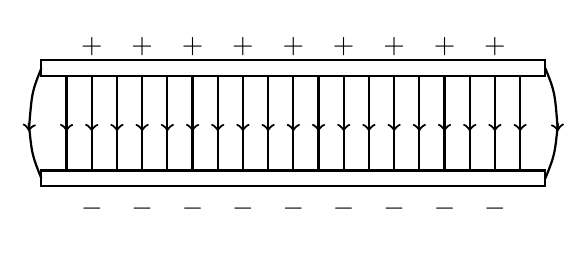
\begin{tikzpicture}[xscale=.8,thick]
      \draw rectangle (8,.2);
      \draw (0,1.4) rectangle (8,1.6);
      \foreach \x in {.4,.8,1.2,...,7.6}{
        \draw[->] (\x,1.4)--(\x,.7);
        \draw (\x,1.4)--(\x,.2);
      }
      \foreach \x in {.8,1.6,2.4,...,7.2}{
        \node at (\x,1.78) {$\bm{+}$};
        \node at (\x,-.28) {$\bm{-}$};
      }
      
      \draw[->] (0,1.5) ..controls(-.15,1.2).. (-.2,.7);
      \draw (-.2,.8) ..controls(-.15,.4).. (0,.1);
      
      \draw[->] (8,1.5) ..controls(8.15,1.2).. (8.2,.7);
      \draw (8.2,.8) ..controls(8.15,.4).. (8,.1);
    \end{tikzpicture}
  \end{center}
  \begin{itemize}
  \item Two plates, each producing an electric field pointing in
    the same direction
  \item The total electric field is twice the value of \emph{one} infinite
    plane, pointing from the positively charged plate toward the negatively
    charged plate

    \eq{-.1in}{
      \boxed{E=\frac\sigma{\epsilon_0}}
    }
  \item $\vec E$ outside the plates is very low (close to zero), except for
    fringe effects at the edges of the plates
  \end{itemize}
\end{frame}



\begin{frame}{Electric Field and Electric Potential Difference}
  Recall the relationship between electric field ($\vec E$) and electric
  potential difference ($V$). If electric field is a function of radial distance
  only, then:
    
  \eq{-.1in}{
    \vec E=-\diff Vr\hat r
  }
  
  This relationship holds regardless of the charge configuration.
\end{frame}




\begin{frame}{Electric Field and Electric Potential Difference}
  \begin{center}
    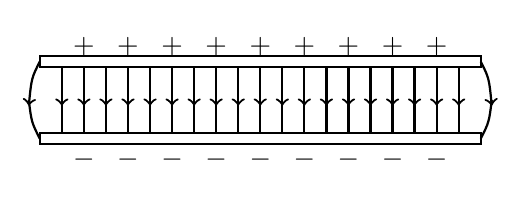
\begin{tikzpicture}[scale=.7,thick]
      \draw rectangle (8,.2);
      \draw (0,1.4) rectangle (8,1.6);
      \foreach \x in {.4,.8,1.2,...,7.6}{
        \draw[->] (\x,1.4)--(\x,.7);
        \draw (\x,1.4)--(\x,.2);
      }
      \foreach \x in {.8,1.6,2.4,...,7.2}{
        \node at (\x,1.78) {$\bm{+}$};
        \node at (\x,-.28) {$\bm{-}$};
      }
        
      \draw[->] (0,1.5) ..controls(-.15,1.2).. (-.2,.7);
      \draw (-.2,.8) ..controls(-.15,.4).. (0,.1);
      
      \draw[->] (8,1.5) ..controls(8.15,1.2).. (8.2,.7);
      \draw (8.2,.8) ..controls(8.15,.4).. (8,.1);
    \end{tikzpicture}
  \end{center}
  In the case of two parallel plates, the electric field is uniform, and the
  relationship simplifies to:

  \eq{-.2in}{
    \boxed{E=\frac{\Delta V}d}
  }
  \begin{center}
    \begin{tabular}{l|c|c}
      \rowcolor{pink}
      \textbf{Quantity} & \textbf{Symbol} & \textbf{SI Unit} \\ \hline
      Electric field intensity & $E$ & \si{\newton\per\coulomb}\\
      Potential difference between plates & $\Delta V$ & \si\volt \\
      Distance between plates       & $d$ & \si\metre
    \end{tabular}
  \end{center}
\end{frame}
\end{document}
